\begin{figure*}[htb]
  \centering
  \begin{subfigure}[t]{0.32\textwidth}
    \centering
    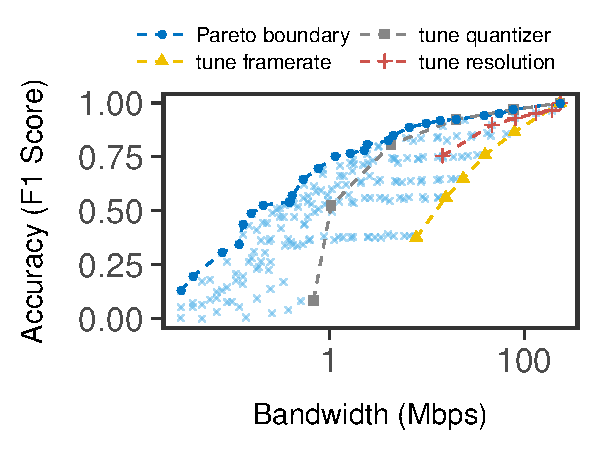
\includegraphics[width=\textwidth]{figures/profile-darknet.pdf}
    \caption{Augmented Reality (AR)}
    \label{fig:ar-profile}
  \end{subfigure}
  \hfill
  \begin{subfigure}[t]{0.32\textwidth}
    \centering
    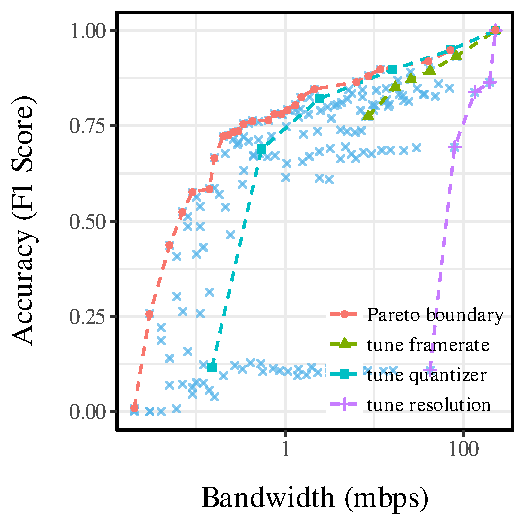
\includegraphics[width=\textwidth]{figures/profile-mot.pdf}
    \caption{Pedestrian Detection (PD)}
    \label{fig:pd-profile}
  \end{subfigure}
  \hfill
  \begin{subfigure}[t]{0.32\textwidth}
    \centering
    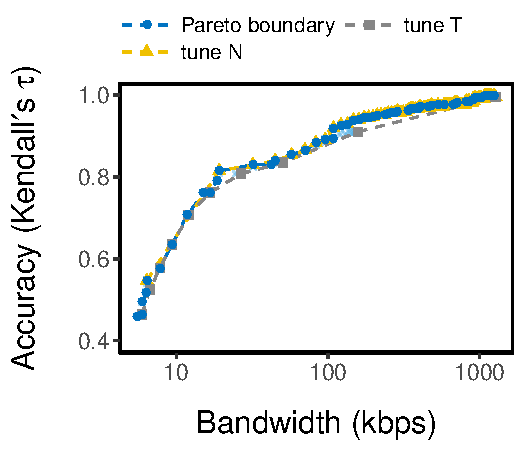
\includegraphics[width=\textwidth]{figures/profile-topk.pdf}
    \caption{Top-K (TK)}
    \label{fig:tk-profile}
  \end{subfigure}
  \caption{Application profiles of three applications. Each cross point is one
    configuration $c$'s performance $(B(c), A(c))$. All figures show the Pareto
    boundary as well as the performance if only tuning one dimension. Note the
    x-axis is in log scale.}
  \label{fig:all-profiles}
\end{figure*}

\section{Evaluation}
\label{sec:evaluation}

In this section, we show the evaluations of \sysname{}, summarizing the results
as follows:

\begin{itemize}[itemsep=0pt, topsep=3pt]
\item[\autoref{sec:application-profiles}] \sysname{} generates Pareto-optimal
  profiles across multiple dimensions with precision
  (\autoref{fig:all-profiles}).
\item[\autoref{sec:online-profiling}] Our parallel and sampling profiling speeds
  up offline and online profiling (\autoref{fig:parallel},
  \autoref{fig:online-tricks}).
\item[\autoref{sec:runtime-adaptation}] At runtime, \sysname{} applications
  achieve sub-second latency and nominal accuracy drop across different network
  conditions (\autoref{fig:ar-runtime}, \autoref{fig:ar-rtt}).
\item[\autoref{sec:multi-task-alloc}] \sysname{} profiles allow different
  resource allocations: resource fairness and utility fairness
  (\autoref{fig:multitask}).
\end{itemize}

\subsection{Application Profiles}
\label{sec:application-profiles}

We run offline profiling using the training dataset described
in~\autoref{tab:apps} and show the learned profiles in
\autoref{fig:all-profiles}. In each figure, the cross dots represent the
bandwidth demand and application accuracy for one configuration. We highlight
the Pareto-optimal boundary $\mathbb{P}$ with blue dashed lines. To understand
each dimension's impact on the degradation, we highlight configurations from
tuning only \textit{one} dimension. From these profiles, we make the following
observations:

\para{Large bandwidth variation.} For all three applications, The bandwidth
requirements of all three applications have two to three orders of magnitude of
difference (note the x-axis is in log scale). For AR and PD, the most expensive
configuration transmits videos at 1920x1080, 30 FPS and 0 quantization; it
consumes 230 mbps. In constrast to the large bandwidth variation, there is a
smaller variation in accuracy. In PD, for example, even after the bandwidth
reduces to 1 mbps (less than 1\% of the maximum), the accuracy is still above
75\%. The large variation allows \sysname{} to operate at a high accuracy
configuration even under severe network deterioration.

\para{Multiple dimensions achieve the optimal.} Comparing dashed lines in each
profile, we see that the Pareto-optimal configurations are only achievable when
multiple knobs are in effect. Tuning only one dimension often leads to
sub-optimal performance. Although TK's Pareto-optimal boundary is aligned with
tuning \texttt{N}, for another dataset with a different distribution, this
behavior will change. \fixme{weak}

\para{Each dimension affects differently}. Within a single profile, the
difference between tuning individual dimensions is evident. For PD, tuning
resolution (the red line) leads to a quicker accuracy drop than tuning frame
rate (the yellow line). Comparing AR and PD, the same dimension has different
impact. Tuning resolution is less harmful in AR than PD; while tuning frame rate
hurts AR more than PD\@. This echoes our initial observation
in~\autoref{sec:making-case-sys-approach} that application- and context-specific
optimizations don't generalize.

% \para{Quantification with precision}. The generated profiles are actionable
% configurations that control the knobs with precision. For example, if PD
% transmits video at 1920x1080 resolution, \(10~\text{FPS}\) and a quantization
% of 20, it will consume 11.7 mbps of bandwidth, achieving roughly 90\%
% accuracy. This saves developers from laboriously analyzing their application
% to compute manual policies.

\subsection{Profiling Efficiency \& Online Profiling}
\label{sec:online-profiling}

This section focuses on the AR application as a case study; our profiling
techniques---parallelism and sampling---do not make assumptions about the
application; therefore, the evaluation results can be generalized to other
applications.

In AR, there are 216 different configurations: 6 resolutions, 6 frame rates and
6 quantization levels. Processing a frame with YOLO~\cite{redmon2016yolo9000} on
GeForce\textregistered\space GTX 970 takes roughly 30 ms.\footnote{YOLO resizes
  an input image to a fixed resolution (416x416) as required by the neural
  network. It takes a similar amount of time to Evaluating each image (with
  different resolutions).} But different configurations require different times
for processing. For example, a \(10~\text{FPS}\) video has 1/3 of the frames to
process in comparison to a \(30~\text{FPS}\) video.  In our experiment, to
evaluate all 216 configurations, it takes 52 seconds for 1-second worth of
data. We denote such overhead as 52X\@. \autoref{sec:automatic-profiling}
discusses techniques to improve the profiling efficiency; we present their
evaluations as follows.

\begin{figure}
  \centering
  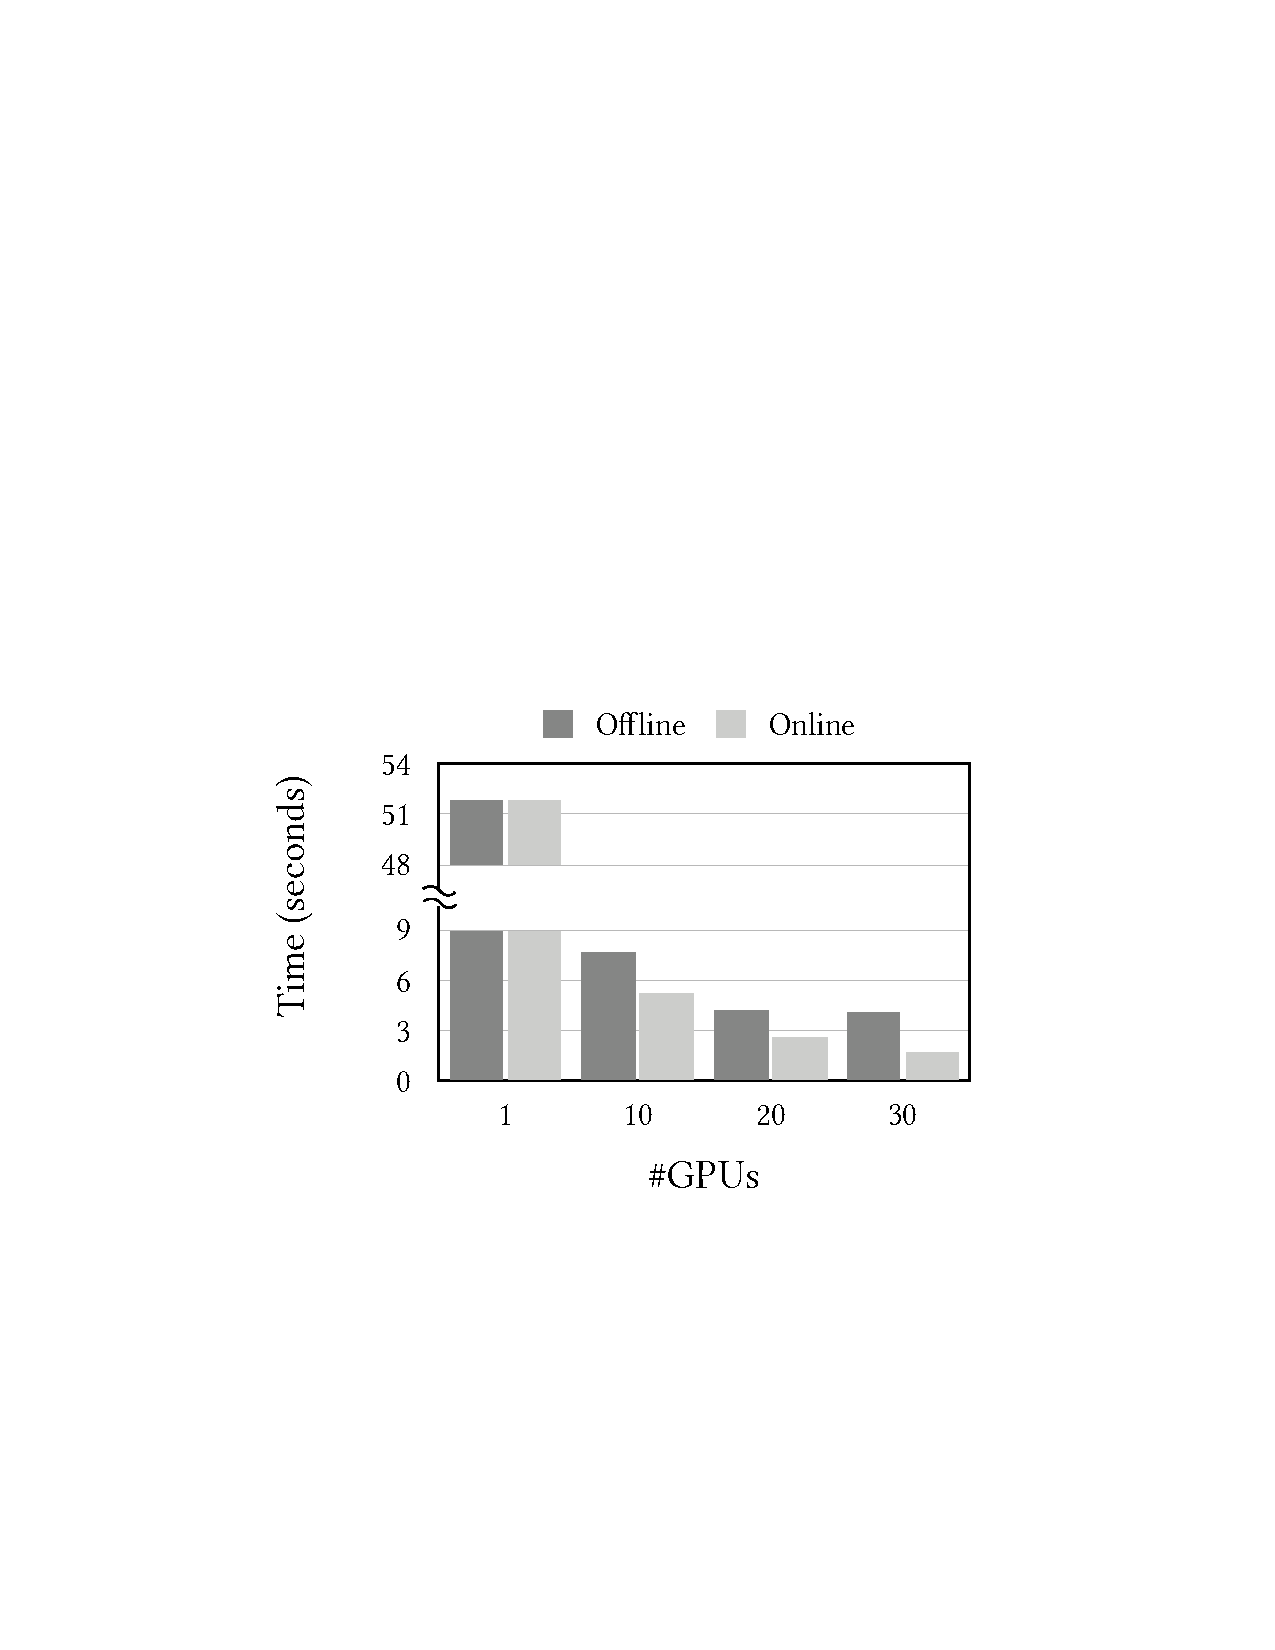
\includegraphics[width=1.0\columnwidth]{figures/parallel.pdf}
  \caption{Parallelism speeds up both offline and online profiling.
  The y-axis shows the profiling time for 1-second video.}
  \label{fig:parallel}
\end{figure}

\para{Parallelism reduces the profiling time (\autoref{fig:parallel})}. Because
evaluating each individual configuration is independent of other configurations,
we parallelize the profiling task by assigning configurations to GPUs.
$(i)$~Our offline profiling assigns configurations randomly.  With the increased
number of GPUs, the overhead reduces from 52X to 4X with 30 GPUs.  $(ii)$~Our
online profiling assigns configurations based on the processing times collected
during offline.  \sysname{} currently uses LFS assignment and can reduce the
overhead to 1.75X with 30 GPUs. \fixme{why?}

\para{Sampling techniques speed up online profiling
  (\autoref{fig:online-tricks}).}
Before we evaluate the speed up, we validate \textit{model drifts} with
real-world data. We use the profile trained in an office environment.  According
to the profile, the application should operate at a configuration of 1280x720
resolution, 30 FPS and a quantization of 20 to meet 11 mbps available bandwidth.
We test it against a home environment, and at about t=100s, the camera points
out of the window to detect objects on the street. Because of the scene change,
the configuration fails to predict runtime bandwidth, as illustrated in
\autoref{fig:offline}.

\begin{figure}
  \centering
  \begin{subfigure}[t]{0.48\columnwidth}
    \centering
    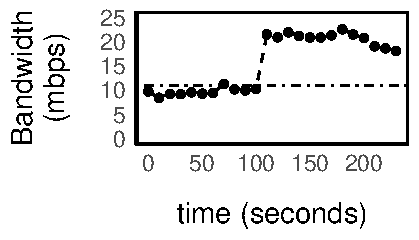
\includegraphics[width=\textwidth]{figures/online1.pdf}
    \caption{Offline only}
    \label{fig:offline}
  \end{subfigure}
  \hfill
  \begin{subfigure}[t]{0.48\columnwidth}
    \centering
    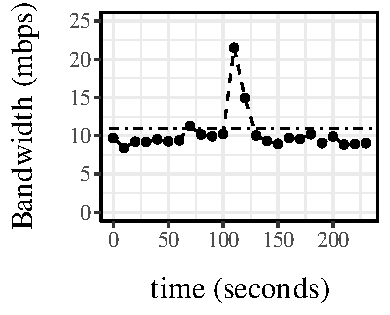
\includegraphics[width=\textwidth]{figures/online2.pdf}
    \caption{Online (continuous)}
    \label{fig:online}
  \end{subfigure}
  \\
  \vspace{1.5em}
  \begin{subfigure}[t]{0.49\columnwidth}
    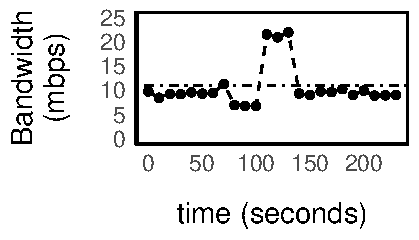
\includegraphics[width=\textwidth]{figures/online3.pdf}
    \caption{Partial data}
    \label{fig:online-partial}
  \end{subfigure}
  \hfill
  \begin{subfigure}[t]{0.49\columnwidth}
    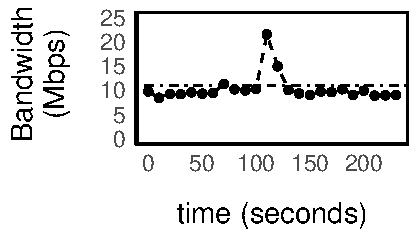
\includegraphics[width=\textwidth]{figures/online4.pdf}
    \caption{Partial configurations}
    \label{fig:online-trigger}
  \end{subfigure}
  \caption{The horizontal reference line is the target bandwidth (11 mbps). (1)
    Online profiling is necessary to handle model drifts ((a) vs.\,(b-d)). (2)
    Sampling techniques---partial data (c) and partial configurations (d)---can
    correct model drifts with less profiling overhead (see
    \autoref{tab:online}), compared to continuous (b).  We omit accuracy
    predictions since in all schemes \sysname{} finds configurations that
    achieve similarly high accuracy (\textasciitilde 90\%).  }
  \label{fig:online-tricks}
\end{figure}

%% Offline: 0
%% Online: 1 frame (1852.21 GPU * seconds)
%% Online (1/10)   (185.2 GPU * seconds)
%% Trigger         ( GPU * seconds)

\begin{table}[t]
  \footnotesize
  \centering
  \begin{tabular}{c c c}
    \toprule
    Online scheme & Overhead & Improvements \\
    \midrule
    Continuous & 52X & Baseline \\
    Partial data & 17X & 3$\times$\\
    Partial configurations & 6X & 8.7$\times$ \\
    \bottomrule
  \end{tabular}
  \caption{Sampling techniques speed up the profiling. We use X to denote the
    overhead of processing one-second worth of data; and $\times$ for the
    improvements. \fixme{Then the baseline should be 1X.}}
  \label{tab:online}
\end{table}

To correct the profile, if we continuously run the profiling online and update
the profile, the application will choose the right configuration to meet the
bandwidth limit.  \autoref{fig:online} shows the bandwidth prediction when we
continuously profile with the past 30 seconds of video. At time t=120s, the new
prediction corrects the drifts. The downside of continuous profiling, as
discussed earlier, is the cost: 52X overhead with 1 GPU\@. In addition to
parallelism, \sysname{} uses two other techniques for online profiling
(improvements in \autoref{tab:online}):

(i) Partial data: Instead of using all the past data, we run profiling with only
a fraction of the raw data.  \autoref{fig:online-partial} shows the bandwidth
prediction \fixme{bandwidth? not prediction?} if we only use 10 seconds of data out
of the past 30 seconds. In this
way, although the profile may be less accurate (the mis-prediction at
t=80--100s), and there is a delay in reacting to data change (the mis-prediction
is corrected after t=125s), we save the online profiling by 3$\times$ (from 52X
to 17X).

(ii) Partial configurations: If we use the past profile as a reference and only
measure a subset of all Pareto-optimal configurations, the savings can be
substantial. A full profiling is only triggered if there is a significant
difference. \autoref{fig:online-trigger} shows the bandwidth prediction if we
evaluate 5 configurations continuously and trigger a full profiling when the
bandwidth estimation is off by 1 mbps or the accuracy is off by 10\%.  For our
test data, this scheme is enough to correct model drifts by predicting an
accurate bandwidth usage (compare \autoref{fig:online} and
\autoref{fig:online-trigger}).  The overhead reduces to 6X because we run full
profiling less often (only two times in this experiment).

Note that these techniques---parallelization, sampling data, and sampling
configurations---can be combined together to further reduce the profiling
overhead. For example, scheduling five GPUs running 5 configurations
continuously to check for model drifts will reduce the overhead to 1X\@. In
practice, the amount of resources to use depends on the budget and the
importance of the job. \sysname{} currently requires developers to configure the
application with proper online profiling techniques.

%% Note that it is not always needed to do online profiling. PD's test data
%% doesn't exhibit model drift.  Nor is online profiling always
%% expensive. Processing TK over all configurations.

\subsection{Runtime Adaptation}
\label{sec:runtime-adaptation}

In this section, we evaluate the runtime performance by controlling available
bandwidth across geo-distributed sites and compare \sysname{} with baselines
including streaming over TCP/UDP, JetStream, and video streaming. Our evaluation
shows that \sysname{} achieves low latency and high accuracy simultaneously
across all applications. Due to space constraints, we only present the result of
AR. The results for PD/TK are in the appendix.

\para{Experiment setup.} We conduct our experiments on four geo-distributed
machines from Amazon EC2, spanning four different regions \fixme{which four?}. Three
act as worker
nodes and one acts as the aggregation server. The average RTTs from worker to
server are 65.2 ms, 22.2 ms, and 50.3 ms.

During the experiment, each worker transmits test data (\autoref{tab:apps}) for
about 10 mins. If the duration of the test data is less than 10 mins, it
loops. Because $B(c_{\max})$ is prohibitively large (raw videos consumes 230
mbps), we use a reasonable configuration to limit the maximum rate. In our AR
experiment, $c_{\max}$ is 1600x900 resolution, \(30~\text{FPS}\) and a
quantization of 20; it consumes about 14 mbps.

Our bandwidth control scheme follows
JetStream~\cite{rabkin2014aggregation}. During the experiment, we use the Linux
\texttt{tc} utility with HTB~\cite{htb, lartc} to control the clients' outgoing
bandwidth. Each experiment involves four phases: $(i)$~before t=200s, there is
no shaping; $(ii)$~at t=200s, we limit the bandwidth to 7.5 mbps for 3 minutes;
$(iii)$~at t=380s, we further decrease the available bandwidth to 5 mbps;
$(iv)$~ at t=440s, we remove all traffic shaping. For UDP, HTB doesn't emulate
the packet loss or out-of-order delivery; so we use \texttt{netem} and configure
the loss probability according to the delivery rate. Because each pair-wise
connection has a different capacity, we impose a \textit{background} bandwidth
limit---25 mbps---to simplify comparisons.

\begin{figure}[t]
  \begin{subfigure}[t]{\columnwidth}
    \centering
    \includegraphics[width=\columnwidth]{figures/runtime_darknet-timeseries.pdf}
    \caption{Time-series plot of the runtime behaviors: throughput (top),
      showing the effect of bandwidth shaping; latency (middle) in log scale;
      and accuracy (bottom).}
    \label{fig:ar-runtime-timeseries}
  \end{subfigure}
  \vspace{1em}
  \\
  \begin{subfigure}[t]{\columnwidth}
    \centering
    \includegraphics[width=\columnwidth]{figures/runtime_darknet-boxplot.pdf}
    \caption{Summary of latency and accuracy during the traffic shaping (between
      t=200s and t=440s). \fixme{not explained.}}
    \label{fig:ar-runtime-boxplot}
  \end{subfigure}
  \caption{Runtime performance. \sysname{} simultaneously achieves low latency
    and high accuracy (with smaller variation). \fixme{not clear in black-white}}
  \label{fig:ar-runtime}
\end{figure}

\para{Baselines.} $(i)$~Streaming over TCP. We re-use \sysname{}'s runtime that
runs over TCP but disable the adaptation. $(ii)$~Streaming over UDP. We use
FFmpeg~\cite{bellard2012ffmpeg} to stream video:
RTP/UDP~\cite{schulzrinne2006rtp} for media and RTSP for
signaling~\cite{schulzrinne1998rtsp}. This is a common setup for video
conferencing and IP cameras~\cite{durresi2005rtp,
  king2009cisco}. $(iii)$~JetStream~\cite{rabkin2014aggregation}. We use the
manual policy described in
\autoref{sec:making-case-sys-approach}. $(iv)$~JetStream++ is a modified version
of JetStream that can use the profile learned by \sysname{}.\footnote{The
  appendix includes details about how we modified JetStream.} $(v)$~HTTP Live
Streaming (HLS). HLS represents a class of HTTP-based adaptive video streaming
techniques. Our setup resembles personalized live streaming
systems~\cite{wang2016anatomy} but uses a smaller chunk for low latency (1
second instead of typical 2-10 seconds).\footnote{The appendix includes details
  about our HLS setup.}

\para{Results.} \autoref{fig:ar-runtime-timeseries} shows the runtime behavior
of \sysname{} and all baselines in time series. \autoref{fig:ar-runtime-boxplot}
summarizes the latency and accuracy with box plots during bandwidth shaping
(between t=200s and t=440s).

The throughput figure shows the effect of traffic shaping. During the shaping,
TCP and UDP make full use of the available bandwidth; in comparison, \sysname{},
JetStream, JetStream++, and HLS are conservative because of adaptation (see
their throughput drops). When we stop the shaping at t=440s, TCP has a
``catch-up'' phase when it's sending all queued items as fast as
possible. JetStream also has queued items because the policy in use (with only
three rules) cannot sustain 5 mpbs bandwidth. \sysname{} increases the
throughput gradually due to the explicit probing phase. HLS is the most
conservative scheme; it does not recover from degradation until t=500s.

The latency figures (both time series and box plot) show that \sysname{} is able
to maintain sub-second latency. During the traffic shaping, TCP queues items at
the sender side for up to hundreds of seconds. In contrast, UDP always transmits
as fast as possible, leading to a consistent low latency.\footnote{FFmpeg
  discards packets that misses a deadline (33ms for 30FPS).} HLS's latency
fluctuates around 2-3 seconds due to chunking, buffering, and network
variations, on par with recent literature~\cite{wang2016anatomy}. Both JetStream
and JetStream++ are able to adapt during traffic shaping. But because
JetStream's runtime reacts instantaneously when the congestion condition
changes, they end up oscillating among polices. \sysname{} effectively addresses
the oscillation with probing and achieves a much lower latency than all
baselines except UDP.

 %   JetStream++        JetStream      Streaming over TCP     AWStream
 %  Min.   :0.04511   Min.   :0.5735   Min.   :0.7179      Min.   :0.6303
 %  1st Qu.:0.82666   1st Qu.:0.7915   1st Qu.:0.8929      1st Qu.:0.8436
 %  Median :0.89385   Median :0.8430   Median :0.9231      Median :0.8942
 %  Mean   :0.84387   Mean   :0.8400   Mean   :0.9153      Mean   :0.8809
 %  3rd Qu.:0.93551   3rd Qu.:0.8969   3rd Qu.:0.9524      3rd Qu.:0.9256
 %  Max.   :0.98947   Max.   :0.9677   Max.   :1.0000      Max.   :0.9849

The two accuracy figures shows that other than UDP, most schemes are able to
maintain high accuracy during the experiment. TCP without adaptation always
sends data at high fidelity, achieving the highest accuracy of \textasciitilde
92\%. But TCP's high accuracy comes with the cost of high latency. JetStream
uses a manual policy that are sub-optimal in comparison to our learned profile,
so its accuracy is low (\textasciitilde 84\%). Using Pareto-optimal
configurations, JetStream++ is able to achieve a higher accuracy
(\textasciitilde 89\%); but because JetStream runtime's policy oscillation, the
accuracy has a large variation. In contrast, \sysname{} chooses configurations
carefully so that it can stay in a steady state as much as possible.  It
achieves a high accuracy of \textasciitilde 89\% with a small variation. HLS
also achieves high accuracy because tuning resolution and encoding quality is
effective in AR. In our PD application where image details matter, HLS's
adaptation leads to a poor accuracy of \textasciitilde 10\% (the figure is in
the appendix).

In summary, \autoref{fig:ar-runtime} shows that \sysname{}'s adaptation achieves
low latency and high accuracy simultaneously. The results during traffic
shaping, in a different form, is shown in \autoref{fig:intro} for discussing the
trade-off between fidelity and freshness.\footnote{We obtain
  \autoref{fig:intro}'s app-specific data by feeding PD's profile to AR.}

\para{Performance with various network delays.} \sysname{} targets at wide area
whose key characteristic is the large variation in
latency~\cite{li2010cloudcmp}. While we've conducted experiments using
real-world setup on Amazon EC2, the latency between EC2 sites is relatively low.
To evaluate how \sysname{} performs with increased network delays, we conducted
another experiment with one pair of client and server under different network
conditions. We use \texttt{netem} to add delays in addition to our bandwidth
shaping. The additional one-way delays ranges from 0ms to 250ms, following a
normal distribution where the variation is 10\% of the added delay, e.g.
$250\pm 25\text{ms}$. We add delays in both direction, so the added RTT can be
as high as 500ms.

\begin{figure}
  \centering
  \includegraphics[width=.9\columnwidth]{figures/runtime_darknet-bench.pdf}
  \caption{\sysname{} maintains low latency and high accuracy under different
    network delay conditions.}
  \label{fig:ar-rtt}
\end{figure}

\autoref{fig:ar-rtt} shows the runtime behavior with various added network
delays. While the latency increases with the added delay, \sysname{} mostly
manages to achieve sub-second latency for all conditions. We see a higher
variation in latency and more outliers as network delay increases. This is
caused by a slow congestion detection when RTT is high. In terms of accuracy,
because \sysname{} mostly stays in \texttt{Steady} state and accuracy only
depends on the level of degradation, \sysname{} achieves similar accuracy for
different network delays.

\subsection{Resource Allocation and Fairness}
\label{sec:multi-task-alloc}
\begin{figure}
  \centering
  \begin{subfigure}[t]{0.8\columnwidth}
    \centering
    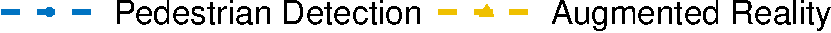
\includegraphics[width=\textwidth]{figures/multitask-legend.pdf}
  \end{subfigure}
  \\
  \vspace{1em}
  \begin{subfigure}[t]{0.45\columnwidth}
    \centering
    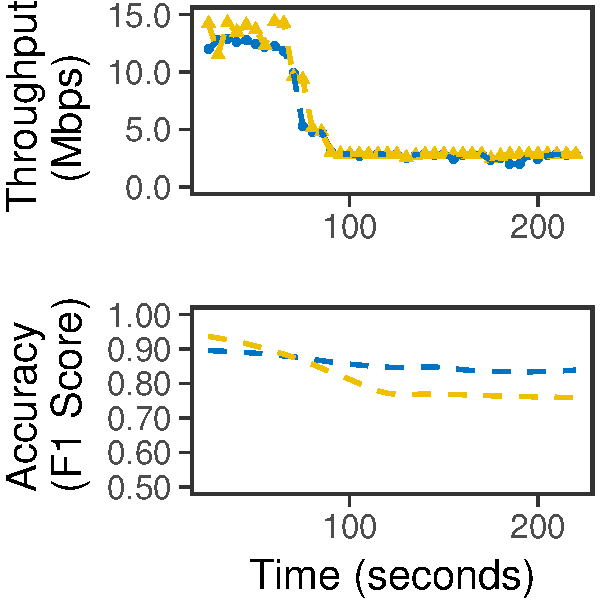
\includegraphics[width=\textwidth]{figures/multitask-left.pdf}
    \caption{Resource Fairness}
    \label{fig:eq-bw}
  \end{subfigure}
  \hfill
  \begin{subfigure}[t]{0.45\columnwidth}
    \centering
    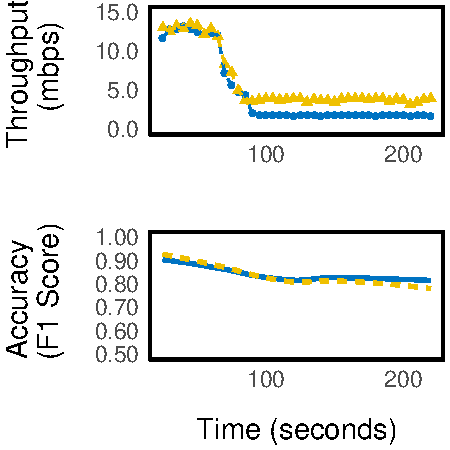
\includegraphics[width=\textwidth]{figures/multitask-right.pdf}
    \caption{Utility Fairness}
    \label{fig:eq-acc}
  \end{subfigure}
  \caption{\sysname{} supports a variety of resource allocation schemes:
    resource fairness (a) and utility fairness (b).}
  \label{fig:multitask}
\end{figure}

We evaluate resource allocations with two applications. In this way, the result
also covers the case of a single application, and can generalize to more
applications.

We choose AR and PD as the example applications.  The clients and servers of
both applications are co-located so that they share the same bottleneck
link. The experiment starts with sufficient bandwidth. At t=60s, we start
traffic shaping to limit the total bandwidth to 6 mbps. When we allocate
resource equally between two applications (\autoref{fig:eq-bw}), each
application gets 3 mbps. Under this condition, PD runs with a higher accuracy of
\textasciitilde 85\% while AR only achieves \textasciitilde 77\%. In addition to
resource fairness, \sysname{} supports utility fairness: it chooses
configurations that maximize the minimal accuracy. In this experiment, PD
receives 2 mbps and AR receives 4 mbps; and both achieve \textasciitilde 80\%
accuracy (\autoref{fig:eq-acc}).

%%% Local Variables:
%%% mode: latex
%%% TeX-master: "../awstream"
%%% End:
